% !TEX root = CartaPerali_Report.tex

\section{Results}
\label{sec:results}

\noindent Regardless of the deployed architecture, we noticed that normalizing our data after computing the MFCC coefficients, the training process gets stuck at a very low accuracy. The model seems to predict always a very small subset of labels regardless of the input data. The reason why this happens is because such normalization discards some important information that is instead necessary to best represent the input audio signal.

\begin{table*}[ht]
	\centering
	\begin{tabular}{c c c c c c c c c}
		\hline
		structure\_id & preprocess\_type & train(s) & prep(s) & load(s) & epochs & tot\_sample & n\_label & acc \\
		\hline
		light\_cnn & specgram & 6880.2 & 3.1 &  2.9 & 50 & 4500000 & 35 & 0.552 \\
		light\_cnn & mfcc     & 2909.6 &  7.8 & 3.0 & 50 & 4500000 & 35 & 0.586 \\
		\hline
	\end{tabular}
	\caption{Preprocessing}
	\label{table:Pr_eprocessing}
\end{table*}

\subsection{\textbf{CNN architectures}}
The tested models's results are provided in Table \ref{table:cnn_performances}:\\
\begin{table}[h!]
\centering
\begin{tabular}{ p{3cm}|p{1.5cm}|p{1.5cm}| }
 \hline
   & Loss & Accuracy\\
\hline
mp & 0\% & 100\%  \\
dd\_relu & 0\% & 100\% \\
dd\_drop & 0\% & 100\% \\
light\_cnn & 0\% & 100\% \\
light\_cnn\_reg\_2 & 0\% & 100\% \\
light\_cnn\_reg\_drop & 0\% & 100\% \\
\hline
\end{tabular}
\caption{CNN Performances}
\label{table:cnn_performances}
\end{table}

\begin{figure}[h]
			\centering
	    	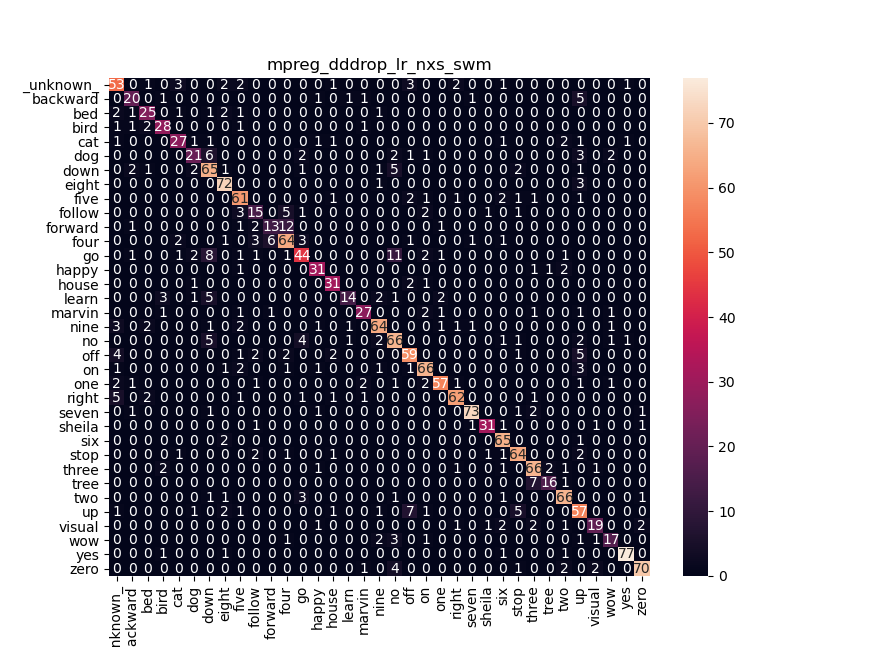
\includegraphics[width=10cm, height=8cm]{conf_matrix_cnn_dii_cm}
	    	\caption{CNN - Confusion matrix}
	    	\label{fig:conf_matrix_cnn}
\end{figure} 



\subsection*{\textbf{Models Comparisons}}
The models are compared in Table \ref{table:comparisons}:\\
\begin{table}[h!]
\centering
\begin{tabular}{ p{3cm}|p{1.5cm}|p{1.5cm}|p{1.5cm} }
 \hline
  & Memory & Time & Parameters \\
\hline\hline
mp & 0\% & 100\% & \\
dd\_relu & 0\% & 100\% & \\
dd\_drop & 0\% & 100\% & \\
light\_cnn & 0\% & 100\% & \\
light\_cnn\_reg\_2 & 0\% & 100\% & \\
light\_cnn\_reg\_drop & 0\% & 100\% & \\
\hline
\end{tabular}
\caption{Models comparisons}
\label{table:comparisons}
\end{table}\\
\noindent From the above results we can observe how {\red{to be continued...}}